
%usepackage es egyebek
\input{common/globdef.tex}

%zarojel, FA...
% ez valahol kellett
\DeclarePairedDelimiter\ceil{\lceil}{\rceil}
\DeclarePairedDelimiter\floor{\lfloor}{\rfloor}

% zárójelek stb.
\newcommand{\Gzjel}[1]{%
{ \left( #1 \right) }
}

\newcommand{\gzjel}[1]{%
{ \left( #1 \right) }
}

\newcommand{\Toligv}[2]{%
#1,\hdots ,#2
}

\newcommand{\GZJ}[1]{%
{ \left( #1 \right) }
}

\newcommand{\KZJ}[1]{%
{ \{ #1 \} }
}

\newcommand{\SZZJ}[1]{%
{ \left[ #1 \right] }
}

\newcommand{\Tolig}[2]{%
#1\hdots #2
}

\newcommand{\SZOR}[2]{%
#1\cdot\hdots\cdot #2
}

% integrál rendes d-vel
\newcommand{\mint}[2]{%
\int #1 \text{d}#2
}

\newcommand{\mder}[2]{%
\frac{\text{d} #1}{\text{d}#2}
}


% ez máshogy van alapban
\newcommand{\tg}[0]{%
\text{tg}
}
\newcommand{\ctg}[0]{%
\text{ctg}
}



% rövidítések
\input{common/szavakdef.tex}

% tcolorbox-al kapcsolatos
\newcommand{\feher}[1]{%
\begin{tcolorbox}[colback=white]
#1
\end{tcolorbox}
}

\newcommand{\zold}[1]{%
\begin{tcolorbox}[colback=green!17]
#1
\end{tcolorbox}
}

\newcommand{\szurke}[1]{%
\begin{tcolorbox}[colback=gray!10!white]
#1
\end{tcolorbox}
}

\newcommand{\szurkeM}[1]{%
\begin{tcolorbox}[colback=gray!10!white, top=-5mm, bottom=3mm]
\begin{gather*}
#1
\end{gather*}
\end{tcolorbox}
}


\newcommand{\sarga}[1]{%
\begin{tcolorbox}[colback=yellow!10!white]
#1
\end{tcolorbox}
}

\newcommand{\barna}[1]{%
\begin{tcolorbox}[colback=brown!20!white]
#1
\end{tcolorbox}
}

\newcommand{\kek}[1]{%
\begin{tcolorbox}[colback=blue!20!white]
#1
\end{tcolorbox}
}

\newcommand{\Fa}[1]{%
\begin{tcolorbox}[colback=brown!20!white]
#1
\end{tcolorbox}
}

\newcommand{\Fnew}[0]{%
\end{tcolorbox}
\begin{tcolorbox}[colback=brown!20!white]
}




\newcommand{\Mo}[1]{%
\begin{tcolorbox}[colback=green!17]
#1
\end{tcolorbox}
}


\newcommand{\Mnew}[0]{%
\end{tcolorbox}
\begin{tcolorbox}[colback=green!17]
}


\newcommand{\egy}[1]{%
\Fa{\input{#1Fa}}
\Mo{\input{#1Mo}}
}


\definecolor{light-gray}{gray}{0.95}
\newcommand{\mcode}[1]{
   \colorbox{light-gray}{\texttt{#1}}
}


% itt van a feladatok listája
\begin{document}\begin{spacing}{1.2}


\input{cim}

   \section*{Tartalom} \label{Tart}
         \nameref{e}\newline
         \nameref{nthroot}\newline
      \newpage
      \section*{az e-szám} \label{e}
      \section*{Tartalom-e} \label{Tarte}
         \nameref{e1}\newline
         \kek{
         \hfill{}\nameref{Tart}
         }\newpage
         \section*{alap} \label{e1}
         \Fa{
            \MatTag{ebase}{
   a_n=\gzjel{ 1+\frac{1}{n}}^{n} \hspace{0.5cm} \nearrow\\
   b_n=\gzjel{ 1+\frac{1}{n}}^{n+1} \hspace{0.5cm} \searrow\\
   a_n < b_m\hspace{1cm} \forall n,m
}
Azaz:
\Mat{
   \exists \lim_{n\to \infty} \gzjel{ 1+\frac{1}{n}}^{n}=\mathrm{e}
}

         }
         \Mo{
         \nameref{e1Mo}
         \hfill\nameref{Tarte}
         }
         \newpage
         \section*{alap-Mo} \label{e1Mo}
         \Mo{
            A \amgm{}miatt:
\szurkeM{
   1\gzjel{ 1+\frac{1}{n}}^{n}<
   \gzjel{\frac{1 + 1+\frac{1}{n}+\cdots+1+\frac{1}{n}}{n+1}}^{n+1}=
   \gzjel{ 1+\frac{1}{n+1}}^{n+1}
}
az $a_n=\gzjel{1+\frac{1}{n}}^{n}$ \szigmon{}nő.


A \gmhm{}miatt:
\szurkeM{
   1\gzjel{ 1+\frac{1}{n}}^{n+1}>
   \gzjel{\frac{n+2}{1 + 1-\frac{1}{n+1}+\cdots+1-\frac{1}{n+1}}}^{n+2}=\\
   =\gzjel{ 1+\frac{1}{n+1}}^{n+2}
}
az $b_n=\gzjel{1+\frac{1}{n}}^{n+1}$ \szigmon{}csökken.
Könnyen látható, hogy:
\szurkeM{
   a_n < b_m \hspace{1cm} \forall m,n \\
   b_n-a_n=\frac{a_n}{n}
}
Mindezek miatt a sorozatok konvergensek és a határértékeik egybeesnek. Ezt
a számot $e$-vel szokták jelölni.

         }
         \Fa{
         \nameref{e1}
         }
         \newpage
      \section*{n-edik gyök} \label{nthroot}
      \section*{Tartalom-nthroot} \label{Tartnthroot}
         \nameref{nthrootSum}\newline
         \nameref{nthroot1}\newline
         \nameref{nthroot2}\newline
         \nameref{nthroot2a}\newline
         \nameref{nthroot3}\newline
         \kek{
         \hfill{}\nameref{Tart}
         }\newpage
         \section*{Summa} \label{nthrootSum}
         \Fa{
            \szurkeM{
   a,b\in \mathbb{R}, \ n\in\mathbb{N}\\
   \forall \ a>0, n>1 \ : \ \exists! \ b>0 \ : \ b^n=a \\
   \text{jele:}\ b=a^{\frac{1}{n}}
}
Tulajdonság:
\szurkeM{
   (a^{\frac{1}{n}})^m=(a^m)^\frac{1}{n}
}

         }
         \Mo{
         \nameref{nthrootSumMo}
         \hfill\nameref{Tartnthroot}
         }
         \newpage
         \section*{Summa-Mo} \label{nthrootSumMo}
         \Mo{
            Legyen $a>1$ és
\szurkeM{
   a_{-}=\{ b\ :\ b^n < a \}\\
   a_{+}=\{ b\ :\ b^n > a \}
}
Megfigyelések:
\begin{itemize}
   \item $a_{-}$ és $a_{+}$ nemüresek
   \item bármely $b\in a_{+}$ felső korlátja $a_{-}$
   \item bármely $b\in a_{-}$ alsó korlátja $a_{+}$
\end{itemize}
A valós számok felső/alsó-határ tulajdonsága miatt egyértelműen létezik
$S=\sup a_{-}$ és $I=\inf a_{+}$ és $S\le I.$
Ha $S < I$ akkor az ábra segít megtalálni az ellentmondást:
\begin{center}
\frame{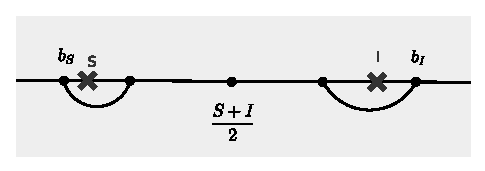
\includegraphics[scale=1.2]{DB/fig/nthroot}}
\end{center}
Tehát $S=I.$ Ezért: $I^n = S^n \le a$ és $I^n\ge a$, vagyis az $S=I$ szám
valóban $a^{\frac{1}{n}}$-ként viselkedik.
%!TODO!


         }
         \Fa{
         \nameref{nthrootSum}
         }
         \newpage
         \section*{konstans} \label{nthroot1}
         \Fa{
            \szurkeM{
   a^{\frac{1}{n}} \to 1 \hspace{1cm} a\in\mathbb{R}
}

         }
         \Mo{
         \nameref{nthroot1Mo}
         \hfill\nameref{Tartnthroot}
         }
         \newpage
         \section*{konstans-Mo} \label{nthroot1Mo}
         \Mo{
            Legyen $a>1$, ekkor valamely $a_n>0$ sorozattal $a^{\frac{1}{n}}=1+a_n$.
A következő megállapításokat tehetjük:
\szurkeM{
   a=\gzjel{1+a_n}^n \ge 1+na_n \hspace{1cm}(\text{Bernoulli})\\
   \frac{a-1}{n}\ge a_n \\
   1\le a^{\frac{1}{n}}\le 1+\frac{a-1}{n}\hspace{1cm}(\text{rendőr-elv})
}
$a<1$ esetén alkalmazzuk $\frac{1}{a}$-ra a fentieket.

         }
         \Fa{
         \nameref{nthroot1}
         }
         \newpage
         \section*{$n$} \label{nthroot2}
         \Fa{
            \Mat{
   \gzjel{ 1-\frac{1}{n}}^{n}\nearrow \frac{1}{\mathrm{e}}\\
   \gzjel{ 1-\frac{1}{n+1}}^{n}\searrow \frac{1}{\mathrm{e}}
}

         }
         \Mo{
         \nameref{nthroot2Mo}
         \hfill\nameref{Tartnthroot}
         }
         \newpage
         \section*{$n$-Mo} \label{nthroot2Mo}
         \Mo{
            A következő megállapításokat tehetjük:
\szurkeM{
   n=\gzjel{1+a_n}^n \ge 1+\frac{n(n-1)}{2}a^2_n \hspace{1cm}(\text{Binomiális})\\
   \sqrt{\frac{2}{n}}\ge a_n \\
   1\le n^{\frac{1}{n}}\le 1+\sqrt{\frac{2}{n}}\\\
   n^{\frac{1}{n}}\to 1 \hspace{1cm}(\text{rendőr-elv})
}

         }
         \Fa{
         \nameref{nthroot2}
         }
         \newpage
         \section*{polinom} \label{nthroot2a}
         \Fa{
            \szurkeM{
   a_0,\hdots,a_m>0\\
   P(n)=\sum_{k=0}^m a_k n^k \\
   P(n)^{\frac{1}{n}}\to 1
}

         }
         \Mo{
         \nameref{nthroot2aMo}
         \hfill\nameref{Tartnthroot}
         }
         \newpage
         \section*{polinom-Mo} \label{nthroot2aMo}
         \Mo{
            Legyen $a=\max\{ a_0,\hdots,a_m \}$:
\szurkeM{
   a_m n^m \le P(n) \le (m+1)an^m \hspace{1cm} (\text{rendőr-elv})
}

         }
         \Fa{
         \nameref{nthroot2a}
         }
         \newpage
         \section*{$n!$} \label{nthroot3}
         \Fa{
            \szurkeM{
   (n!)^{\frac{1}{n}} \to \infty
}

         }
         \Mo{
         \nameref{nthroot3Mo}
         \hfill\nameref{Tartnthroot}
         }
         \newpage
         \section*{$n!$-Mo} \label{nthroot3Mo}
         \Mo{
            A \amqm{}és egyszerű átalakítás mutatja:
\szurkeM{
   \gzjel{\frac{\sum{\frac{1}{k}}}{n}}^2\le
   \frac{\sum{\frac{1}{k^2}}}{n}\le
   \frac{\sum{\frac{2}{k(k+1)}}}{n}=
   2\frac{1-\frac{1}{n+1}}{n}\le\frac{2}{n}
}
A \gmhm{ből:}
\szurkeM{
   (n!)^{\frac{1}{n}} \ge \frac{n}{\sum\frac{1}{k}}\ge
   \sqrt{\frac{n}{2}}
}

         }
         \Fa{
         \nameref{nthroot3}
         }
         \newpage

\end{spacing}
\end{document}

